\documentclass[11pt,twoside]{article}
\usepackage{informat}
\usepackage{epsfig}

\begin{document}
  \title{Title of the paper}
   \author{NameOfAuthor1 SurnameOfAuthor1, Name2 Surname2 and Name3 Surname3 \\
      Institution1 Address\\
      E-mail1 and WebAddress1 \\
      \AndAuthor
      Name4 Surname4 \\
      Institution2 Address\\
      E-mail2 and WebAddress2}
  \titleodd{Title of the\ldots}
  \authoreven{N. SurnameofAuthor1 et al.}
  \keywords{keyword1, keyword2, keyword3}
  \received{June 24, 2013}

  \abstract{Text of the abstract. Typically around 10 sentences.}
  \abstractSi{}

  \maketitle

\section{Introduction}
Text of the introduction.

\section{Second section title}
Second section text.

\begin{table}[h]
  \begin{center}
  \begin{tabular}{|c|c|c|} \hline
    Comp. & Start no. & End no. \\ \hline
    1 & 4 & 12 \\ \hline
    3 & 5 & 12 \\ \hline
    5 & 1 & 7  \\ \hline
    7 & 1 & 4  \\ \hline
  \end{tabular}
  \end{center}
  \caption{Title of the table}
\end{table}

\subsection{First subsection of the second section title}
First subsection text.

\begin{figure}[htb]
  \begin{center}
    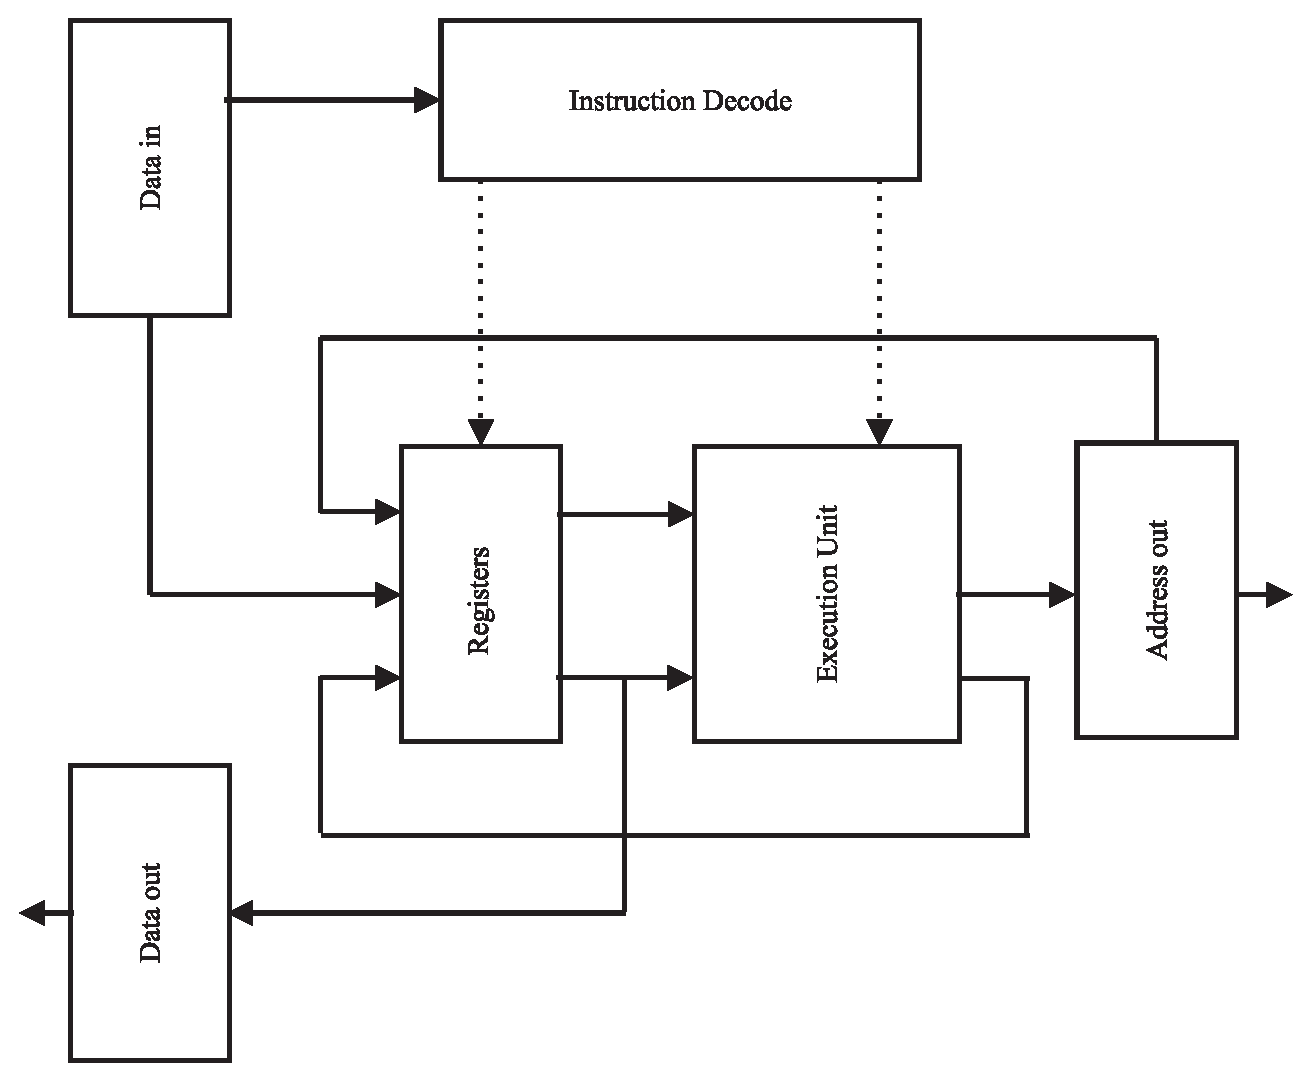
\epsfig{file=author1.eps,width=75mm} % figure1.eps is a standalone file in EPS format
  \end{center}
  \caption{Caption of the figure.}
\end{figure}

\begin{figure*}[b] % '*' for two columns
  \begin{center}
    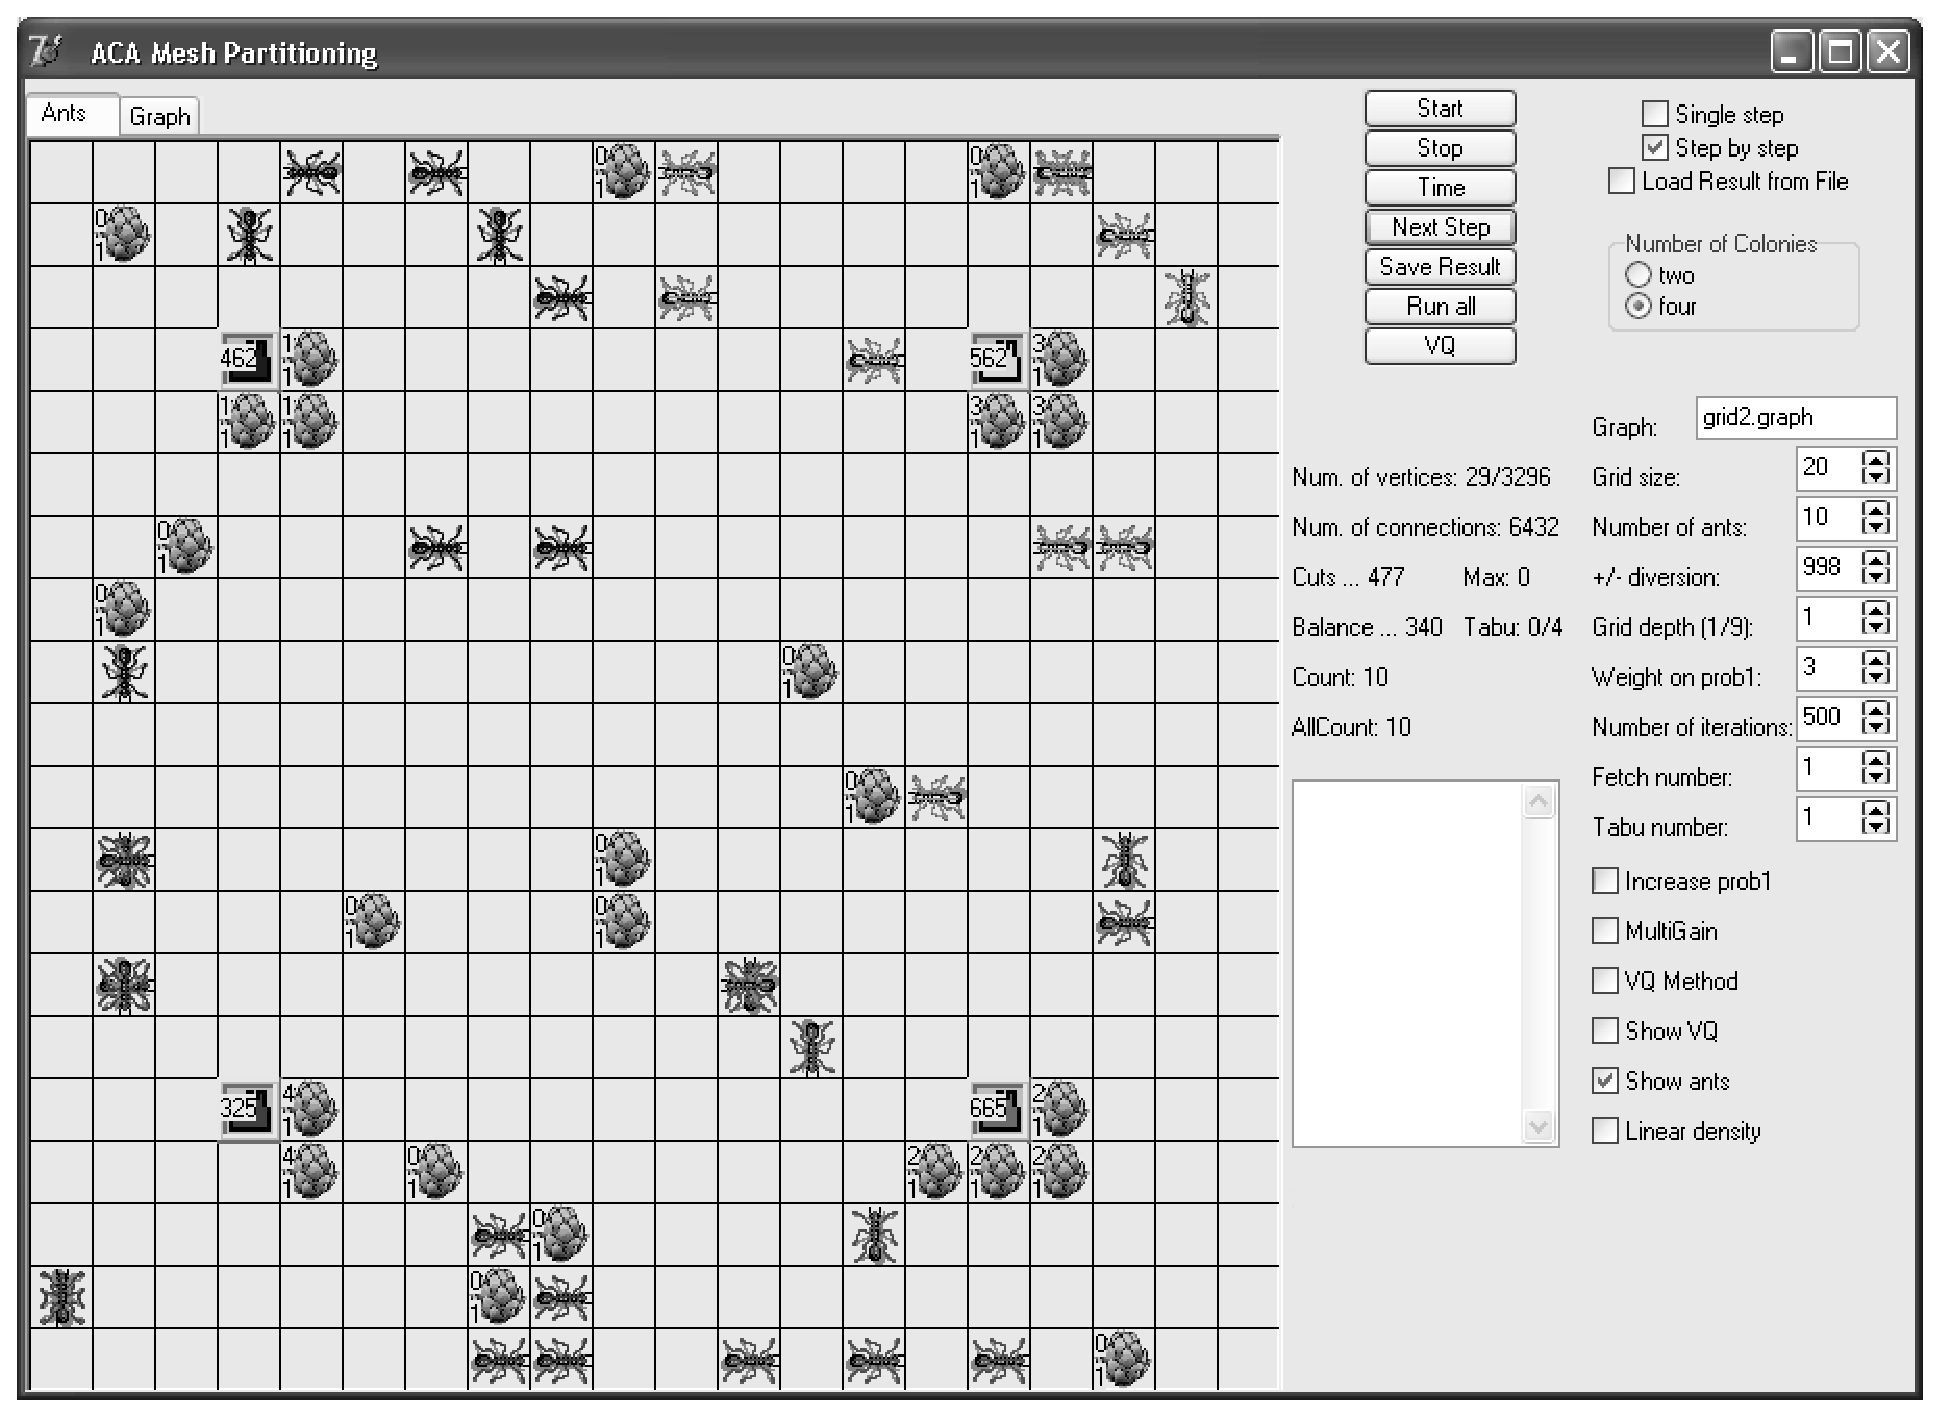
\epsfig{file=author2.eps, width=160mm} % figure2.eps is a standalone file in EPS format
  \end{center}
  \caption{Caption of the figure 2 over two columns.}
\end{figure*}

\section{Conclusion} % conclusion and discussion; just discussion etc.
Conclusion text.

\subsection*{Acknowledgement}
Acknowledgement text.

% bibliography style is not predefined; authors can apply their own,
% but it should be sent to matjaz.gams@ijs.si with the accepted paper
\begin{thebibliography}{99}

  % book
  \bibitem{} Author (year) {\it Title of the book}, Publisher.

  % journal paper
  \bibitem{} Author (year) Title of the paper, {\it Title of the journal}, Publisher, pp. nn--mm.

  % conference
  \bibitem{} Author (year) Title of the paper, {\it Title of the proceedings}, Publisher, Location, pp. nn--mm.

\end{thebibliography}

\end{document}
